Throughout this section, let $(\cC,\cE)$ denote a geometric setup equipped with a presentable six-functor formalism
\[
\cD '\colon\Span{\cC}_{\cE}\longrightarrow\Prlst
\]
in the sense of~\cite[App~A.5]{Mann2022}. We assume for simplicity that $\cC$ contains all finite limits, so that $\cD '$ is a lax symmetric monoidal functor, where $\Span{\cC}_{\cE}$ is equipped with the symmetric monoidal structure described in~\cite[Rem~A.5.5]{Mann2022}. It follows formally that $\cD '(\pt )$ has a canonical commutative algebra structure and that $\cD '$ factors through a symmetric monoidal functor
\[
  \cD\colon\Span{\cC}_{\cE}\longrightarrow\pPrl{\cD '(\pt )}.
\]
(Note that $\cD (X)$ has the same underlying presentable stable $\infty$-category as $\cD '(X)$.) We will assume the following:
\begin{enumerate}[label=(\Alph*)]
\item\label{monoidality-assumption} The functor $\cD$ is a symmetric monoidal functor, i.e.~the canonical functor
  \[
    \cD (X)\otimes_{\cD(\pt )}\cD (Y)\longrightarrow\cD(X\times Y)
  \]
  is an equivalence for each pair of objects $X$ and $Y$ in $\cC$.
\end{enumerate}
\begin{notation}
  For the remainder of this section, we let $\mdef{\cA} = \cD (\pt )$.
\end{notation}
Assumption~\labelcref{monoidality-assumption} is satisfied for the six-functor formalisms that interest us in this paper, such as the six-functor of sheaves of on locally compact Hausdorff spaces and of local systems on anima.\Onote{Find reference for the fact that it fails for \'etale sheaves}
\subsection{The categorified Lefschetz trace formula}

The starting point is the following observation about dualizable
objects in span categories:
\begin{lem}
  If $X\in \cC$ is admissible,
  then $X \in \Span{\cC}_{\cE}$ is self-dual (and in particular dualizable), with evaluation and unit given by the spans
  \[X\xleftarrow{\id} X \xrightarrow{\Delta} X\times X\,, \quad
    \pt \xleftarrow{} X \xrightarrow{\id} X\,\]
  respectively, and counit and coevaluation given by the flipped spans.
\end{lem}
% We assume further that
% \begin{itemize}
% \item[(M)]\label{ass: monoidal} The lax symmetric monoidal structure on $\mathcal D\colon\Span{\mathcal C}_{\mathcal E}\to\mathrm{Pr}^{\mathrm{L}}_{\mathcal A}$ exhibits $\mathcal D$ as a (strong) symmetric monoidal functor.
% \end{itemize}
% We also fix an object $X\in\mathcal C$, and assume that
% \begin{itemize}
% \item[(S)]\label{ass: seperated} The projection to the terminal object $X\to\pt$ is admissible.
% \end{itemize}
% We refer to an object satisfying (S) as \tdef{separated}.
% \\
% Since admissible morphisms are stable under base-change, the diagonal morphism $\Delta\colon X\to X\times X$ of a separated object is also admissible. This implies that $X$ is self-dual as an object of $\Span{\mathcal C}_{\mathcal E}$ \todo{REF, universality of spans?}, 
% \[
%   \begin{tikzpicture}[baseline=(current bounding box.center)]
%     \node (X) at (0,1){$X$};
%     \node (pt) at (-1,0){$\pt $};
%     \node (XX) at (1,0){$X\times X$};

%     \draw (X) edge[->] (pt);
%     \draw (X) edge[->] node[very near start,right=3pt]{{\small $\Delta$}}(XX);
%   \end{tikzpicture}
%   \qquad\text{and}\qquad
%   \begin{tikzpicture}[baseline=(current bounding box.center)]
%     \node (X) at (0,1){$X$};
%     \node (pt) at (1,0){$X .$};
%     \node (XX) at (-1,0){$X\times X$};

%     \draw (X) edge[->] (pt);
%     \draw (X) edge[->] node[very near start,left=3pt]{{\small $\Delta$}}(XX);
%   \end{tikzpicture}
% \]

Using our assumption~\labelcref{monoidality-assumption}, we deduce that $\cD (X)$ is dualizable as an object of $\pPrl{\cA}$ for each admissible $X\in\cC$. In particular, for an endofunctor $F\colon\cD (X)\to\cD (X)$, we can take the trace $\tr{F\curvearrowright\cD (X)}{\pPrl{\cA}}$. The first incarnation of the Lefschetz trace formula that we consider is a description of this trace when $F$ is a pullback functor $f^*$ for some endomorphism $f\curvearrowright X$ in $\cC$.

\begin{prop}[Categorified trace formula]\label{thm:categorical-fixed-pts}
Let $\cD\colon \Span{\cC}_{\cE}\to \pPrl{\cA}$ be a symmetric monoidal,
$\cA$-linear six-functor formalism and let $X\in \cC$ be admissible.
  For every endomorphism $f\colon X\to X$, we have that
  \begin{equation}
    \label{eq:categorical-trace-formula}
    \tr{f^*\curvearrowright\mathcal D (X)}{\mathrm{Pr}^{\mathrm{L}}_{\mathcal A}}\simeq (X^f)_!(X^f)^* \in \Map_{\pPrl{\cA}}(\cA,\cA)\,,
  \end{equation}
  where $X^f\in\mathcal C$ is defined by the pullback
  \begin{equation}
    \label{eq:pullback-defn-of-fixedpts}
    \begin{tikzcd}
      X^f  & X \\
      X & X\times X\,.
      \arrow[from=1-1, to=1-2]
      \arrow["\lrcorner",phantom,very near start, from=1-1, to=2-2]
      \arrow[from=1-1, to=2-1]
      \arrow["\Delta", from=1-2, to=2-2]
      \arrow["{(\id ,f)}"', from=2-1, to=2-2]
    \end{tikzcd}
  \end{equation}
  If additionally $f\colon X\to X$ is admissible, we moreover have
    \begin{equation}
    \label{eq:categorical-trace-formula-exceptional}
    \tr{f_!\curvearrowright\mathcal D (X)}{\mathrm{Pr}^{\mathrm{L}}_{\mathcal A}}\simeq (X^f)_!(X^f)^*.
  \end{equation}
\end{prop}
\begin{proof}
  Recall that $f^*$ is the result of applying the symmetric monoidal functor $\mathcal D\colon \Span{\mathcal C}_{\mathcal E} \to \pPrl{\cA}$ to the span
  \begin{equation}
    \label{eq:pullback-in-correspondence}
    \begin{tikzpicture}[baseline=(current bounding box.center)]
      \node (X) at (-1,0){$X$};
      \node (Z) at (0,1){$Y$};
      \node (Xprime) at (1,0){$Y,$};

      \draw (Z) edge[->] node[very near start,left=3.5pt]{{\footnotesize $f$}}(X);
      \draw (Z) edge[double equal sign distance] (Xprime);
    \end{tikzpicture}
  \end{equation}
  Since symmetric monoidal functors preserve traces by \cref{lem: sym mon preserve trace}, we get a natural equivalence
  \[
    \tr{f^*\colon \D{X}\to \D{X}}{}\simeq\D{\tr{X\xleftarrow{f} X\xrightarrow{\id} X}{}},
  \]
  where the trace of $X\xleftarrow{\id} X\xrightarrow{f} X$ is taken in the span category $\Span{\mathcal C}_{\mathcal E}$. Using the description of the evaluation and coevaluation on $X$ from the discussion preceding the theorem, we then find that the trace of the morphism~\eqref{eq:pullback-in-correspondence} in the span category is given by the outer span in the diagram:
  % \[
  %   \begin{tikzpicture}[baseline=(current bounding box.center)]
  %     \node (X) at (0,1){$X$};
  %     \node (pt) at (-1,0){$\pt $};
  %     \node (XX) at (1,0){$X\times X$};

  %     \draw (X) edge[->] (pt);
  %     \draw (X) edge[->] node[very near start,right=3pt]{{\small $\Delta$}}(XX);
  %   \end{tikzpicture}
  %   \qquad\text{and}\qquad
  %   \begin{tikzpicture}[baseline=(current bounding box.center)]
  %     \node (X) at (0,1){$X$};
  %     \node (pt) at (1,0){$\pt $,};
  %     \node (XX) at (-1,0){$X\times X$};

  %     \draw (X) edge[->] (pt);
  %     \draw (X) edge[->] node[very near start,left=3pt]{{\small $\Delta$}}(XX);
  %   \end{tikzpicture}
  % \]
  % respectively. The trace of $X\xleftarrow{\id} X\xrightarrow{f} X$ is therefore the outer span in the diagram
  \begin{equation}
    \label{eq:trace-in-span-category}
    \begin{tikzpicture}[baseline=(current bounding box.center),scale=2]
      %%% Nodes
      % bottom row (R0)
      \node (R0C0) at (-3,0){$\pt$};
      \node (R0C2) at (-1,0){$X\times X$};
      \node (R0C4) at (1,0){$X\times X$};
      \node (R0C6) at (3,0){$\pt$,};

      % R1
      \node (R1C1) at (-2,1){$X$};
      \node (R1C3) at (0,1){$X\times X$};
      \node (R1C5) at (2,1){$X$};

      % R2
      \node (R2C2) at (-1,2){$P$};
      \node[rotate=-45] (pullback1) at (-1,1.7){{\large $\lrcorner$}};
      \node (R2C4) at (1,2){$X$};
      \node[rotate=-45] (pullback1) at (1,1.7){{\large $\lrcorner$}};

      % R3
      \node (R3C3) at (0,3){$P^{\prime}$};
      \node[rotate=-45] (pullback1) at (0,2.7){{\large $\lrcorner$}};

      %%% Edges
      % Towards left
      \draw
      (R3C3) edge[->] (R2C2)
      (R2C2) edge[->] (R1C1)
      (R1C1) edge[->] (R0C0);

      \draw (R2C4) edge[->] node[near start,left=3pt]{{\small $\Delta$}} (R1C3)
      (R1C3) edge[->] node[near start ,left=3pt]{{\small $f\times\id$}} (R0C2);

      \draw (R1C5) edge[->] node[near start,left=3pt]{{\small $\Delta$}} (R0C4);

      % Towards right
      \draw
      (R3C3) edge[->] (R2C4)
      (R2C4) edge[double distance=1.5pt] (R1C5)
      (R1C5) edge[->] (R0C6);

      \draw
      (R2C2) edge[->] (R1C3)
      (R1C3) edge[double distance=1.5pt] (R0C4);

      \draw (R1C1) edge[->] node[near start,right=3pt]{{\small $\Delta$}} (R0C2);
    \end{tikzpicture}
  \end{equation}
  where by the pasting law the top corner $P'$ can be computed as the pullback~\eqref{eq:pullback-defn-of-fixedpts}, i.e. there is a canonical equivalence $P'\simeq X^f$. Note also that $X^f$ is separated since $X^f\to X$ is pulled back from $\Delta\colon X\to X\times X$ and thus admissible, whence the composition $X^f\to X\to\pt$ is admissible.

  If $f$ is admissible, the equation~\eqref{eq:categorical-trace-formula-exceptional} follows by dualizing~\eqref{eq:categorical-trace-formula}, which interchanges $({-})^*$ and $({-})_!$.
\end{proof}

\begin{rmk}\label{rmk:utopian-lefschetz}
  Note that \cref{thm:categorical-fixed-pts} looks like a utopian version of the Lefschetz trace formula from topology; it says that for any map $f\curvearrowright X$, the trace of the induced map on the categorified cohomology $\mathcal D(X)$ is isomorphic to the compactly-supported cohomology of the fixed points $X^f$. This lacks several subtleties that are present in the actual Lefschetz trace formula. For instance, the theorem neither has a transversality assumption on $f$ nor fixed point indices to correct for the lack of transversality, and there is no compactness/properness assumption on $X$. These subtleties arise from the failure of~\labelcref{eq:categorical-trace-formula} to decategorify nicely.

  Assume for simplicity that $\cA = \Sp$, as in the case of sheaves on locally compact Hausdorff spaces or local systems on anima. The naive approach to decategorification here is to apply topological Hochschild homology
  \[
    \THH\colon\Prdual\too\Sp
  \]
  on both sides of the formula. On the left-hand side, one would then want to relate $\THH$ of $\tr{f^*\curvearrowright\cD (X)}{}$ to the trace of map induced by $f$ on $\THH(\cD (X))\simeq\Gamma_c(X;\SS )$. If $\cD (X)$ were dualizable \emph{as an object of $\Prdual$}, this would be formal, since $\THH$ is symmetric monoidal and thus preserves traces of endomorphisms of dualizable objects. However, for a dualizable category to be dualizable \emph{in} dualizable categories (aka \tdef{fully dualizable} or \tdef{fully saturated}) is very restrictive. Indeed,~\cite{Harr2026} shows that the category of sheaves $\Shv (\tset ;\Sp )$ on a locally compact Hausdorff space $\tset$ is fully dualizable if and only if $\tset$ is a finite set of points. The failure of $\cD (X)$ to be fully dualizable also means that there is no formal reason to expect the trace of $f^*$ to be strongly continuous, even if $f^*$ is; and hence no reason for $\THH$ to even be \emph{defined} for the (equivalent) functors appearing in~\labelcref{eq:categorical-trace-formula}. Indeed, a generic self-homeomorphism of a manifold is known to have a Cantor set of fixed points~\cite{Craciun2013}, in which case the functor $(X^f)_!(X^f)^*\simeq\SS^{\oplus\aleph_0}\otimes{-}$ will fail very badly to be strongly continuous. Similar subtleties surrounding decategorification and commuting $\THH$ with trace also play a central role in~\cite{Beraldo_Pippi2024}.
\end{rmk}
\subsection{Naturality}
It will be useful to know that~\labelcref{eq:categorical-trace-formula} is a \emph{natural} equivalence in the situations that we care about. For this to make sense, we must have a functoriality in mind for both the left and right sides of the equation. This functoriality is brought to you by 2-categorical enhancements of the six-functor formalism $\cD$ \`a la \cite{Cnossen_Lenz_Linskens2026} and the higher trace machinery of~\cite{Hoyois_Scherotzke_Sibilla2017}, as we now explain.

Suppose that $\cD '$ is (equivalent to the six-functor formalism) constructed as in~\cite{Liu_Zheng2012,Mann2022} from the data of a suitable decomposition $(\cI,\cP)$ of $\cE$ \cite[Def~A.5.9]{Mann2022} and a lax symmetric monoidal functor $\cD ''\colon\cC^{\op}\to\Prlst$, such that the tuple $(\cC ,\cE ,\cI ,\cP ,\cD '')$ satisfies the conditions of~\cite[Prop~A.5.10]{Mann2022}. \cite{Cnossen_Lenz_Linskens2026} define a symmetric monoidal $(\infty ,2)$-categorical enhancement of the span category $\Span{\cC}_{\cE}$, denoted $\mdef{\sSpan{\cC}_{\cE,\cI,\cP}}$, with 2-morphisms from $X\leftarrow Z\to Y$ to  $X\leftarrow Z'\to Y$ given by spans of spans
\begin{equation}
  \label{eq:span-of-spans}
  \begin{tikzpicture}[baseline=(current bounding box.center)]
    \node (X) at (-1.5,0){$X$};
    \node (Z) at (0,1.5){$Z$};
    \node (Zprime) at (0,-1.5){$Z',$};
    \node (W) at (0,0){$W$};
    \node (Y) at (1.5,0){$Y$};

    \draw (Z) edge[->] (Y);
    \draw (Z) edge[->] (X);
    \draw (Zprime) edge[->] (Y);
    \draw (Zprime) edge[->] (X);
    \draw (W) edge[->] node[near start,left=1.5pt]{{\footnotesize $f$}}(Z);
    \draw (W) edge[->] node[near start,left=1.5pt]{{\footnotesize $i$}}(Zprime);
  \end{tikzpicture}
\end{equation}
where $i\in\cI$ and $f\in\cP$. (See Definition 4.10 and the discussion on page 50 of op.~cit.~for a formal construction of $\sSpan{\cC}_{\cE ,\cI ,\cP}$ and its symmetric monoidal structure.) The main theorem of op.~cit.~promotes $\cD '$ to a lax symmetric monoidal 2-functor
\begin{equation*}
  \widetilde\cD'\colon\sSpan{\cC}_{\cE,\cI,\cP}^{\otimes}\too\Prlstf,
\end{equation*}
which on $(\infty ,1)$-categorical cores is equivalent to $\cD '$. Our assumption~\labelcref{monoidality-assumption} implies that $\widetilde\cD '$ factors through a symmetric monoidal functor
\begin{equation}
  \label{eq:2-categorical-sixff}
  \widetilde\cD'\colon\sSpan{\cC}_{\cE,\cI,\cP}\too\pPrlf\cA,
\end{equation}
where $\pPrlf\cA$ is the $(\infty ,2)$-category of $\cA$-linear stable categories. It follows from~\cite[Thm~1.7]{Hoyois_Scherotzke_Sibilla2017} that there is a commutative diagram
\begin{equation}
  \label{eq:naturality-of-lefschetz}
  \begin{tikzcd}
    \Endtrl (\sSpan{\cC}_{\cE,\cI,\cP})\arrow[d,"\Trc"]\arrow[r]
    & \Endtrl (\pPrlf\cA )\arrow[d,"\TrcL"]\\
    \Omega_{\pt} \sSpan{\cC}_{\cE,\cI,\cP}\arrow[r]
    & \Omega_{\cA} \pPrlf\cA.
  \end{tikzcd}
\end{equation}
On \emph{objects}, the commutativity of this diagram recovers the equivalence~\labelcref{eq:categorical-trace-formula}. That is, the counterclockwise composition sends a span of the form
\[X\xleftarrow fX\xrightarrow{\id}X
\]to $(X^f)_!(X^f)^*\colon\cA\to\cA$, whereas the clockwise composition spits out $\tr{f^*\curvearrowright\cD (X)}{}$. The counterclockwise resp.~clockwise composition in the diagram therefore implement the functoriality for the left-hand side resp. right-hand side of~\labelcref{eq:categorical-trace-formula}, and the invertible 2-cell filling the commutative diagram implements a natural equivalence between these functors.

We already know how the clockwise composition in~\labelcref{eq:naturality-of-lefschetz} behaves on morphisms, see~\cref{sec: trace theory}. As for the counterclockwise composition, we first observe
\begin{prop}
  Let
  \[
    \Lambda =
    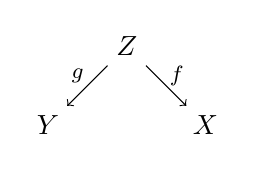
\begin{tikzpicture}[baseline=(current bounding box.center)]
      \node (X) at (1,0){$X$};
      \node (Z) at (0,1){$Z$};
      \node (Y) at (-1,0){$Y$};

      \draw (Z) edge[->] node[near start,left=1.5pt]{{\footnotesize $g$}} (Y);
      \draw (Z) edge[->] node[near start,right=1.5pt]{{\footnotesize $f$}} (X);
    \end{tikzpicture}
  \]
  be a 1-morphism in $\sSpan{\cC}_{\cE ,\cI ,\cP}$ with both $f$ and $g$ admissible, and suppose that
  \begin{enumerate}[label=(\roman*)]
  \item $f$ is \'etale and the diagonal map $\Delta_f\colon Z\to Z\times_XZ$ is proper; and
  \item $g$ is proper and the diagonal map $\Delta_g\colon Z\to Z\times_YZ$ is \'etale.
  \end{enumerate}
  Then
    \[
    \Lambda '=
    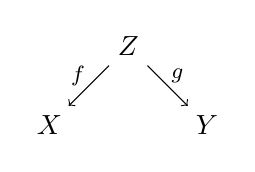
\begin{tikzpicture}[baseline=(current bounding box.center)]
      \node (X) at (-1,0){$X$};
      \node (Z) at (0,1){$Z$};
      \node (Y) at (1,0){$Y$};

      \draw (Z) edge[->] node[near start,right=1.5pt]{{\footnotesize $g$}} (Y);
      \draw (Z) edge[->] node[near start,left=1.5pt]{{\footnotesize $f$}} (X);
    \end{tikzpicture}
  \]
  is an internal right adjoint to $\Lambda$.
\end{prop}
\begin{proof}
  Note that
  \[
    \Lambda \circ\Lambda '=
    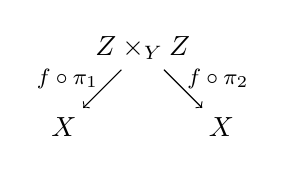
\begin{tikzpicture}[baseline=(current bounding box.center)]
      \node (X) at (1,0){$X$};
      \node (Z) at (0,1){$Z\times_YZ$};
      \node (Y) at (-1,0){$X$};

      \draw (Z) edge[->] node[near start,left=1.5pt]{{\footnotesize $f\circ\pi_1$}} (Y);
      \draw (Z) edge[->] node[near start,right=1.5pt]{{\footnotesize $f\circ\pi_2$}} (X);
    \end{tikzpicture}
    \qquad\text{and}\qquad
    \Lambda '\circ\Lambda =
    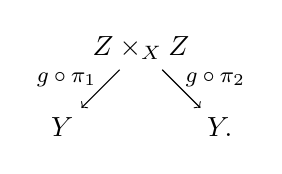
\begin{tikzpicture}[baseline=(current bounding box.center)]
      \node (X) at (1,0){$Y.$};
      \node (Z) at (0,1){$Z\times_XZ$};
      \node (Y) at (-1,0){$Y$};

      \draw (Z) edge[->] node[near start,left=1.5pt]{{\footnotesize $g\circ\pi_1$}} (Y);
      \draw (Z) edge[->] node[near start,right=1.5pt]{{\footnotesize $g\circ \pi_2$}} (X);
    \end{tikzpicture}
  \]
  By assumption, we have the following 2-morphisms in $\sSpan{\cC}_{\cE ,\cI ,\cP}$.
  \[
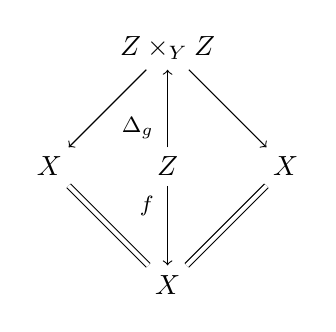
\begin{tikzpicture}[baseline=(current bounding box.center)]
    \node (X) at (-1.5,0){$X$};
    \node (Z) at (0,1.5){$Z\times_YZ$};
    \node (Zprime) at (0,-1.5){$X$};
    \node (W) at (0,0){$Z$};
    \node (Y) at (1.5,0){$X$};

    \draw (Z) edge[->] (Y);
    \draw (Z) edge[->] (X);
    \draw (Zprime) edge[double distance=1.5pt] (Y);
    \draw (Zprime) edge[double distance=1.5pt] (X);
    \draw (W) edge[->] node[near start,left=1.5pt]{{\footnotesize $\Delta_g$}}(Z);
    \draw (W) edge[->] node[near start,left=1.5pt]{{\footnotesize $f$}}(Zprime);
  \end{tikzpicture}
  \qquad\text{and}\qquad
  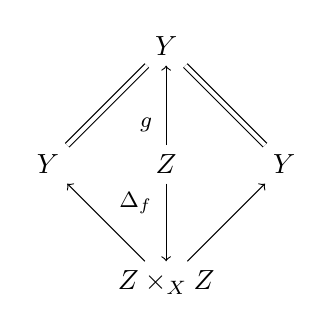
\begin{tikzpicture}[baseline=(current bounding box.center)]
    \node (X) at (-1.5,0){$Y$};
    \node (Z) at (0,-1.5){$Z\times_XZ$};
    \node (Zprime) at (0,1.5){$Y$};
    \node (W) at (0,0){$Z$};
    \node (Y) at (1.5,0){$Y$};

    \draw (Z) edge[->] (Y);
    \draw (Z) edge[->] (X);
    \draw (Zprime) edge[double distance=1.5pt] (Y);
    \draw (Zprime) edge[double distance=1.5pt] (X);
    \draw (W) edge[->] node[near start,left=1.5pt]{{\footnotesize $\Delta_f$}}(Z);
    \draw (W) edge[->] node[near start,left=1.5pt]{{\footnotesize $g$}}(Zprime);
  \end{tikzpicture}
\]
from $\Lambda \circ\Lambda '$ to $\id$ and $\id$ to $\Lambda '\circ\Lambda $, respectively. It is straightforward to check that these 2-morphisms satisfy the triangle equality, and hence witness an adjunction $\Lambda \circ\Lambda '\dashv \Lambda '\circ\Lambda$ as desired.
\end{proof}
\begin{cor}
  Let $X\in\cC$ be an admissible object.
  \begin{enumerate}[label=(\alph*)]
  \item The 1-morphism $Y\xleftarrow f X\xrightarrow\id X$ has an internal right adjoint if $f$ is proper and $\Delta_f\colon X\to X\times_Y X$ is \'etale.
  \item The 1-morphism $X\xleftarrow{\id} X\xrightarrow f Y$ has an internal right adjoint if $X$ is \'etale and $\Delta_f\colon X\to X\times_Y X$ is proper.
  \end{enumerate}
\end{cor}
\Onote{Write that the map on traces induced by a lax comm square in span-category with internally left adjoint horizontal arrows (i.e.~a map in traceable endos) is induced by the associated map on fixed points.}
\subsection{Decategorification}
Following~\cite{Kondyrev_Prikhodko2020,Ben-Zvi_Nadler2021}, we decategorify~\cref{thm:categorical-fixed-pts} by using the functoriality of trace in traceable endomorphisms to produce for a suitable endomorphism $f\curvearrowright X$ in $\cC$ a commutative triangle in $\cA$ whose base implements the ``Lefschetz trace'' of $f$, and whose legs implement fixed point indices for $f$, c.f.~\cref{rmk:utopian-lefschetz}. For this we will make the following additional assumption about our six-functor formalism:
\begin{enumerate}[label=(\Alph*)]
  \setcounter{enumi}{1}
\item\label{locally-rigid-assumption} $\cA$ is locally rigid.
\end{enumerate}
\begin{defn}[Lefschetz trace]
  Let $X\in\cC$ be an admissible object, and suppose that $X_*X^*\mathbf 1\in\cA$ is dualizable. The \tdef{Lefschetz trace} of an endomorphism $f\curvearrowright X$, denoted $\mdef{\ch{}{f}}$, is the trace of the induced map $f^*\curvearrowright X_*X^*\mathbf 1$ in $\cA$.
\end{defn}
\begin{prop}[The Lefschetz trace formula]
  Let $X\in\cC$ be an admissible object, and suppose that $X$ is suave and prim. Then the Lefschetz trace $\ch {} f$ is defined, and there is a commutative diagram
  \begin{equation}
    \label{eq:abstract-lefschetz-triangle}
    \begin{tikzcd}[column sep=small]
      & (X^f)_!(X^f)^*\mathbf 1\arrow[dr]\\
      \mathbf 1\arrow[rr,swap,"\ch {} f"]\arrow[ru] & & \mathbf 1.
    \end{tikzcd}
  \end{equation}
  Furthermore,
  \begin{enumerate}[label=(\alph*)]
  \item \Onote{Identify legs if assumptions are satisfied}
  \end{enumerate}
\end{prop}
\begin{exam}[The topological Lefschetz formula]
  Consider the six-functor formalism 
\end{exam}
\begin{exam}[The homotopical Reidemeister trace]
  
\end{exam}
\begin{exam}[The parametrized homotopical Reidemeister trace]
  Let $B$ be a locally compact Hausdorff space such that the $\infty$-topos $\Shv (B)$ is hypercomplete. There is a symmetric monoidal functor
  \[
    \Shv (B)^\op\too\Prlst
  \]
  given informally by
  \[
    F\mapsto \Shv (\Shv (B)_{/F};\Sp ).
  \]
  \Onote{In fact such a functor exists for any $\infty$-topos; there should be plently of places to cite for the slice $\infty$-topos defining a functor from $\cB$ into topoi, and then we are just post-composing this with the usual sheaf functor. The hypercompleteness is used to check the conditions for construction a six-functor formalism stalkwise.}
\end{exam}
%%% Local Variables:
%%% mode: LaTeX
%%% TeX-master: "main"
%%% End:
